\documentclass[varwidth=true, border=2pt]{standalone}
\usepackage{amsmath,amssymb}% math symbols / fonts
\usepackage{pgfplots}
\usetikzlibrary{decorations.markings}
\pgfplotsset{compat=newest}

\begin{document}
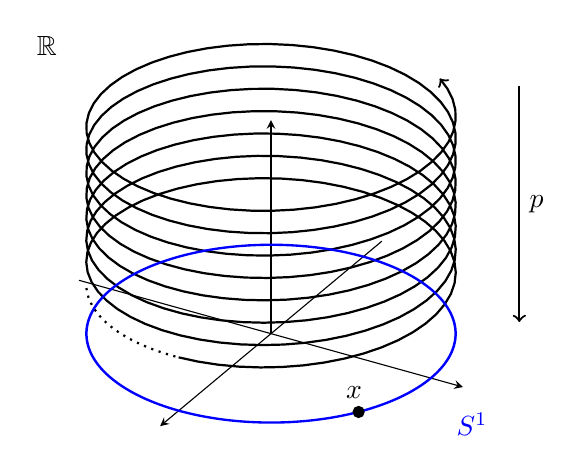
\begin{tikzpicture}
\draw[->, thick] (7,5) -- (7, 2) node [midway, right] {$p$};
\node at (1,5.5) {$\mathbb{R}$} ;
\node at (6.4,0.7) {$\color{blue} S^1$};
\node at (4.9,1.1){$x$};
\begin{axis}[
 view={-30}{-45},
 axis lines=middle,
 zmax=60,
 height=8cm,
 xtick=\empty,
 ytick=\empty,
 ztick=\empty,
 enlarge y limits=true,
 enlarge x limits=true,
]

\addplot3+[->,ytick=\empty,yticklabel=\empty,
  mark=none,
  thick,
  black,
  domain=0:14.8*pi,
  samples=400,
  samples y=0,
]
({sin(deg(x))},{cos(deg(x)},{x+15});
\addplot3+[ytick=\empty,yticklabel=\empty,
  mark=none,
  thick,
  dotted,
  black,
  domain=-1:0,
  samples=100,
  samples y=0,
]
({sin(deg(x))},{cos(deg(x)},{x+15});

\addplot3+[,ytick=\empty,yticklabel=\empty,
  mark=none,
  thick,
  blue,
  domain=0:14.7*pi,
  samples=400,
  samples y=0,
]
({sin(deg(x))},{cos(deg(x)},{0});

%%%%%%%%%%%%% Point
\addplot3+[
  mark options={color=black},
  mark=*
]
coordinates {({sin(deg(45)},{cos(deg(45))},0)};
%%%%%%%%%%%%%

\end{axis}
\end{tikzpicture}
\end{document}
